\documentclass[a4paper]{article}

%% Language and font encodings
\usepackage[english]{babel}
\usepackage[utf8]{inputenc}
\usepackage[T1]{fontenc}

%% Sets page size and margins
\usepackage[a4paper,top=3cm,bottom=2cm,left=3cm,right=3cm,marginparwidth=1.75cm]{geometry}

%% Useful packages
\usepackage{amsmath}
\usepackage{graphicx}
\usepackage[colorinlistoftodos]{todonotes}
\usepackage[colorlinks=true, allcolors=blue]{hyperref}

\newcommand{\github}{https://github.com/kauron/etsinf3/tree/master/CPA/lab2}

\title{CPA Lab 2}
\author{Carlos Santiago Galindo Jiménez\\Jesús Vélez Palacios}

\begin{document}
\maketitle
\section{Objective}
Parallelize the execution of a program that reconstructs an image whose rows have been shuffled. Study different approaches and some improvements to the algorithm.

Examine the temporal cost for each version for different amounts of threads. Detail also the speedup and efficiency.

\section{Exercises\protect\footnotemark }
\footnotetext{All files are provided in the appropriate task. However, the files are also hosted on \href{\github}{GitHub}. These files will be exactly equal to those sent. Some references even link to a certain line in the file, for greater clarity.}
\begin{description}
    \item [\texttt{\href{\github /src/encaja-e1.c\#L167}{encaja-e1.c}}] Time the method encaja. Completed with two calls to \texttt{omp\_get\_wtime()}.
    \item [\texttt{encaja-e2-p?.c}] Parallelize the different loops (if at all possible).
    \begin{description}
        \item [\texttt{i}] This loop will never be parallelizable, because each line depends on the previous one.
        \item [\texttt{j}] This loop can be parallelized protecting the variables with \texttt{private(x, distancia)}. The last \texttt{if} must be protected as \texttt{critical section} and the condition has to be rechecked after entering it. \href{\github /src/encaja-e2-pJ.c\#L118}{Source code}
        \item [\texttt{x}] This loop can also be parallelized, and needs a \texttt{reduction(+:distancia)} to compute the distance correctly. \href{\github /src/encaja-e2-pX.c\#L120}{Source code}
    \end{description}
    \item [\texttt{\href{\github /src/encaja-e3.c\#L122}{encaja-e3.c}}] Improve the program by exiting loop \texttt{x} if the partial sum surpasses the current minimum. Solved adding an \texttt{if} that breaks from the loop in that case.
    \item [\texttt{encaja-e4-p?.c}] Parallelize \texttt{encaja-e3.c} in the loops that are viable.
    \begin{description}
        \item [\texttt{j}] This loop is parallelized in the same way as in exercise 2. \href{\github /src/encaja-e4-pJ.c\#L118}{Source code}
        \item [\texttt{x}] This loop needs the most work. It must be parallelized as a \texttt{parallel} block. The first iteration is assigned to \texttt{omp\_get\_thread\_num()} and each thread increments \texttt{x} by \texttt{omp\_get\_num\_threads()}. It still needs a \texttt{reduction} for \texttt{distancia}. \href{\github /src/encaja-e4-pX.c}{Source code}
    \end{description}
\end{description}

\section{Performance}
\subsection{Expected results}
\subsubsection*{Exercise 2: encaja-e2}
In general, the outer loops will achieve better parallel performance than inner loops. This is due to the overhead of creating a thread, meaning the extra resources the system spends creating and \todo{wording here?} destroying the threads.
There is a point where the overhead becomes so great that there is no speedup. For this reason it is expected that \texttt{encaja-e2-pJ.c} ($n$ threads) will perform better than \texttt{encaja-e2-pX.c} ($n^2$ threads).
\subsubsection*{Exercise 3: encaja-e3}
The change proposed should mean an improvement in time required to recover the image.
\subsubsection*{Exercise 4: encaja-e4}
In this case, the same should happen as in exercise 2: \texttt{encaja-e4-pJ} should run faster than \texttt{encaja-e4-pX}. It is more difficult to compare each with the rest of iterations.

\subsection{Testing}
All the programs have been run and timed in the Kahan Cluster, from the university. The job submission file for that system is provided along with the source code as \texttt{\href{\github /encaja.sh}{encaja.sh}}. This file executes all the exercises, and prints the results in \texttt{csv} format (values separated by commas) for easier data processing. A \texttt{\href{\github /Makefile}{Makefile}} is also included with the source code, because \texttt{encaja.sh} makes use of it.

\subsection{Results: time required}
The sequential programs (\texttt{encaja-e1.c} and \texttt{encaja-e3.c}) have only been tested once.
The parallel programs have been run with 2, 4, 8, 16 and 32 threads to test their performance.
As shown in the graph\footnote{The data in the graph for $nodes=1$ is the timing from the sequential versions of the program (\texttt{encaja-e1.c} and \texttt{encaja-e3.c})} from Figure \ref{fig:graph-time}, loop \texttt{j} achieves much better results that loop \texttt{x}.
On top of that, the improvement implemented in the exercises 3 and 4 pays off in the sequential version and loop \texttt{j}, but in loop \texttt{x} there is practically no difference with \texttt{encaja-e2-pX}.
In the latter case, the overhead of the threads gets so big that the algorithm gets slower.

\begin{figure}[h]
    \centering
    \begin{tabular}{l r}
        Program            & Execution time \\ \hline
        \texttt{encaja-e1} & 15.257217      \\
        \texttt{encaja-e3} &  2.725587      \\ \hline
    \end{tabular}
    \caption{Sequential execution times}
    \label{fig:table-time-seq}
\end{figure}
\begin{figure}[h]
    \centering
    \begin{tabular}{l r r r r r}
        Program               & 2t        & 4t        & 8t        & 16t        & 32t        \\ \hline
        \texttt{encaja-e2-pJ} & 6.938746  & 3.548883  & 1.970450  & 1.183996   &  0.726187  \\
        \texttt{encaja-e4-pJ} & 1.439842  & 0.795035  & 0.496000  & 0.330912   &  0.256960  \\
        \texttt{encaja-e2-pX} & 8.337415  & 5.464151  & 5.557857  & 8.197272   & 12.789012  \\
        \texttt{encaja-e4-pX} & 4.065065  & 4.217589  & 5.164125  & 8.656438   & 13.590685  \\ \hline
    \end{tabular}
    \caption{Parallel execution times}
    \label{fig:table-time}
\end{figure}
\begin{figure}[h]
    \centering
    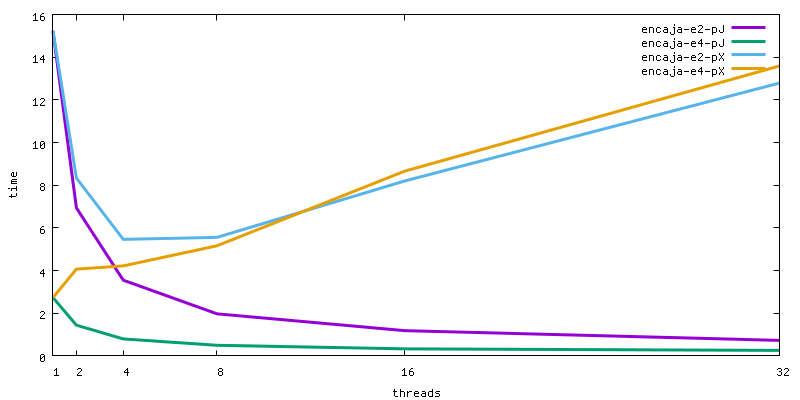
\includegraphics[width=\textwidth]{../img/time}
    \caption{Threads --- \unskip \, time graph }
    \label{fig:graph-time}
\end{figure}


\subsection{Results: speedup}
The speedup of a parallel program respect to the sequential version is the improvement in speed due to the parallelization. It is computed as:
\begin{equation}
S(n,p)=\frac{t(n)}{t(n,p)}
\end{equation}
Applying the previous formula with $t(n)=t_{encaja-e1}$ and $t(p,n)$ equal to the table in Figure \ref{fig:table-time} we obtain Figure \ref{fig:table-speedup}. Values $S(n) > 1$ indicate an improvement and values $S(n) < 1$ signal a worsening in the performance. All values are $>1$, therefore there is improvement in all cases. The highest result is obtained on \texttt{encaja-e4-pJ}, with a $5830\%$ speedup.
\begin{figure}[h]
    \centering
    \begin{tabular}{l r r r r r}
        Program               & 2t       & 4t       & 8t       & 16t      & 32t      \\ \hline
        \texttt{encaja-e2-pJ} &  2.19624 &  4.29407 &  7.73384 & 12.87090 & 20.98510 \\
        \texttt{encaja-e4-pJ} & 10.58390 & 19.16790 & 30.72410 & 46.05190 & 59.30550 \\
        \texttt{encaja-e2-pX} &  1.82780 &  2.78893 &  2.74191 &  1.85905 &  1.19158 \\
        \texttt{encaja-e4-pX} &  3.74881 &  3.61323 &  2.95096 &  1.76044 &  1.12129 \\ \hline
    \end{tabular}
    \caption{Speedup}
    \label{fig:table-speedup}
\end{figure}

The speedup can also be computed with $t(n)=t_{encaja-e3}$, in order to compare exercise 4 its sequential version (activity 3). 

In this table it can be appreciated that the loop \texttt{x} has all values $S(n,p)<0$, and therefore provides no improvement the sequential code in \texttt{encaja-e3.c}. The apparent betterment shown in Figure \ref{fig:table-speedup} is respect to the initial program. The threads --- \unskip \, time graph in Figure \ref{fig:graph-time} clearly shows that the performance of \texttt{encaja-e4-pX.c} (yellow) is below all other versions.

\begin{figure}[h]
    \centering
    \begin{tabular}{l r r r r r}
        Program               & 2t       & 4t       & 8t       & 16t      & 32t       \\ \hline
        \texttt{encaja-e4-pJ} & 1.898620 & 3.438490 & 5.511530 & 8.261170 & 10.638700 \\
        \texttt{encaja-e4-pX} & 0.672491 & 0.648171 & 0.529368 & 0.315802 &  0.201147 \\ \hline
    \end{tabular}
    \caption{Speedup of \texttt{encaja-e4} respect to \texttt{encaja-e3}}
    \label{fig:table-speedupR3}
\end{figure}

\begin{figure}[h]
    \centering
    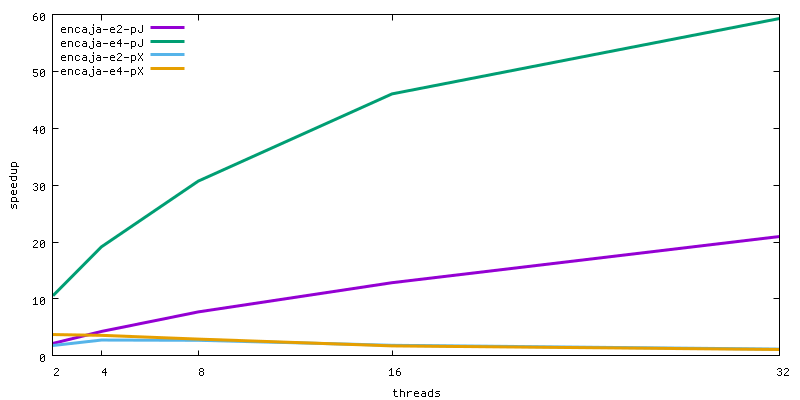
\includegraphics[width=\textwidth]{../img/speedup}
    \caption{Threads --- \unskip \, speedup graph}
    \label{fig:graph-speedup}
\end{figure}

\subsection{Results: efficiency}
The efficiency of a parallel program is defined as:
\begin{equation}
E(n,p)=\frac{S(n,p)}{p}
\end{equation}
where $p$ is the number of threads and $S(n,p)$ the speedup previously computed. Figure \ref{fig:table-efficiency} shows the efficiency values for exercises 2 and 4. This metric means \todo{complete this}

\begin{figure}[h]
	\centering
	\begin{tabular}{l r r r r r}
		Program 			  & 2t  	& 4t 	   & 8t 	  & 16t      & 32t 		\\ \hline
		\texttt{encaja-e2-pJ} & 1.09812 & 1.073520 & 0.966730 & 0.804431 & 0.655784	\\
		\texttt{encaja-e4-pJ} & 5.29195 & 4.791970 & 3.840510 & 2.878240 & 1.853300	\\
		\texttt{encaja-e2-pX} & 0.91390 & 0.697233 & 0.342739 & 0.116191 & 0.037237 \\
		\texttt{encaja-e4-pX} & 1.87441 & 0.903308 & 0.368870 & 0.110028 & 0.035040 \\ \hline
	\end{tabular}
	\caption{Efficiency}
	\label{fig:table-efficiency}
\end{figure}
\begin{figure}[h]
    \centering
    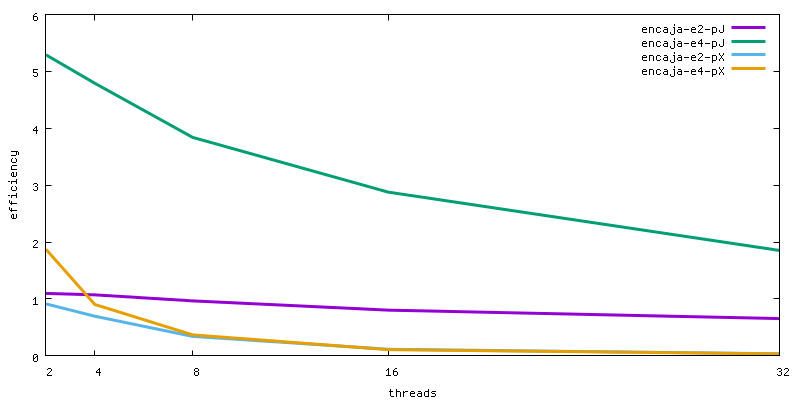
\includegraphics[width=\textwidth]{../img/efficiency}
    \caption{Threads --- \unskip \, efficiency graph}
    \label{fig:graph-efficiency}
\end{figure}

\section{Conclusions}
This lab practice is an extensive walk-through of OpenMP and parallelization practices and techniques. In this weeks we have learned that:
\begin{itemize}
    \item Some loops can be parallelized, some cannot.
    \item Thread overhead may become a problem with inner loops.
    \item Clever changes to sequential algorithms can outperform simpler parallel ones.
    \item Appropriate control structures for critical sections and shared, private variables.
\end{itemize}
\todo[inline]{write conclusions}


\end{document}

